\documentclass{article}
\usepackage{import}
\usepackage{tcolorbox}
\usepackage{amsmath}
\usepackage{amssymb}
\usepackage{amsthm}
\usepackage{geometry}
\usepackage{enumitem}
\usepackage{pdfpages}
\usepackage{transparent}
\usepackage{booktabs}
\usepackage{bm}
\usepackage{tabularx}
\usepackage{multirow}
% \usepackage{minted}
\usepackage{xcolor}
\usepackage{setspace}
\usepackage[hidelinks]{hyperref}
\usepackage{pgfplots}
% \usepackage{soulpos}

\tcbuselibrary{theorems}
\tcbuselibrary{skins}

\setcounter{tocdepth}{6}
\setcounter{secnumdepth}{6}

\newcommand{\param}{\boldsymbol{\theta}}
\newcommand{\bs}{\boldsymbol}
\newcommand{\data}{\mathcal D}

% pgfplots settings
\pgfplotsset{compat=1.18}
\usepgfplotslibrary{external}

% tabularx Settings
\renewcommand\tabularxcolumn[1]{>{\centering\arraybackslash}m{#1}}

% Page Settings
\newgeometry{vmargin={15mm}, hmargin={15mm, 15mm}}
\setlength{\parindent}{0pt}
\setlength{\parskip}{0.7\baselineskip}%{0.8em plus 1pt minus 1pt}

\onehalfspacing

% hyperref Settings
\hypersetup{
    colorlinks=true,
    linkcolor=blue,
    filecolor=magenta,      
    urlcolor=cyan,
}

% inkscape Settings
\newcommand{\incfig}[1]{%
    \def\svgwidth{\columnwidth}
    \import{./figure/}{#1.pdf_tex}
}

% inline code block settings
\newtcbox{\mybox}[1][]{
    on line,
    arc=1pt, outer arc=2pt,
    colback=lightgray!50!white, colframe=lightgray!50!white,
    boxsep=0pt, left=0pt, right=-1pt, top=2pt, bottom=0pt,
    boxrule=0pt, #1
}

\NewDocumentCommand{\code}{v}{%
  \begingroup\ttfamily
  \codeulinner{#1}%
  \endgroup%
}

% Definition Box Styles
\newtcbtheorem[auto counter, number within=subsection]{defn}{Definition}{
% basic settings
    theorem name and number,
    separator sign={},
    description delimiters={(}{)},
    enhanced jigsaw,
    sharp corners,
% box margins and rules
    boxrule=1pt,
    left=0.2cm,right=0.2cm,top=0.2cm,
    toptitle=0.1cm,
    bottomtitle=0.08cm,
% box colors
    colframe=white!25!black,
    colback=white,
    coltitle=white,
% box fonts
    fonttitle=\bfseries,fontupper=\normalsize
}{defn}

% Theorem Box Styles
\newtcbtheorem[auto counter, number within=subsection]{thm}{Theorem}{
% basic settings
    theorem name and number,
    separator sign={},
    description delimiters={(}{)},
    enhanced jigsaw,
    sharp corners,
% box margins and rules
    boxrule=1pt,
    left=0.2cm,right=0.2cm,top=0.2cm,
    toptitle=0.1cm,
    bottomtitle=0.08cm,
% box colors
    colframe=white!25!black,
    colback=white,
    coltitle=white,
% box fonts
    fonttitle=\bfseries,fontupper=\normalsize
}{thm}

% Lemma Box Styles
\newtcbtheorem[number within=tcb@cnt@thm]{lem}{Lemma}{
% basic settings
    theorem name and number,
    separator sign={},
    description delimiters={(}{)},
    enhanced jigsaw,
    sharp corners,
% box margins and rules
    boxrule=1pt,
    left=0.2cm,right=0.2cm,top=0.2cm,
    toptitle=0.1cm,
    bottomtitle=0.08cm,
% box colors
    colframe=white!50!black,
    colback=white,
    coltitle=white,
% box fonts
    fonttitle=\bfseries,fontupper=\normalsize
}{lem}

% Corollary Box Styles
\newtcbtheorem[number within=tcb@cnt@thm]{cor}{Corollary}{
% basic settings    
    theorem name and number,
    separator sign={},
    description delimiters={(}{)},
    enhanced jigsaw,
    sharp corners,
% box margins and rules
    boxrule=1pt,
    left=0.2cm,right=0.2cm,top=0.2cm,
    toptitle=0.1cm,
    bottomtitle=0.08cm,
% box colors
    colframe=white!50!black,
    colback=white,
    coltitle=white,
% box fonts
    fonttitle=\bfseries,fontupper=\normalsize
}{cor}

% Remark Box Styles
\newtcbtheorem[number within=subsection]{rem}{Remark}{
% basic settings
    theorem name and number,
    separator sign={},
    description delimiters={(}{)},
    enhanced jigsaw,
    sharp corners,
% box colors
    colframe=white!60!black,
    colback=white,
    coltitle=black,
% box margins and rules
    boxrule=1pt,
    left=0.2cm,right=0.2cm,top=0.2cm,
    toptitle=0.1cm,
    bottomtitle=0.08cm,
% box fonts
    fonttitle=\bfseries,fontupper=\normalsize
}{rem}

% Example Box Styles
% Remark Box Styles
\newtcbtheorem[number within=subsection]{exm}{Example}{
% basic settings
    theorem name and number,
    separator sign={},
    description delimiters={(}{)},
    enhanced jigsaw,
    sharp corners,
% box colors
    colframe=white!60!black,
    colback=white,
    coltitle=black,
% box margins and rules
    boxrule=1pt,
    left=0.2cm,right=0.2cm,top=0.2cm,
    toptitle=0.1cm,
    bottomtitle=0.08cm,
% box fonts
    fonttitle=\bfseries,fontupper=\normalsize
}{exm}


% Proof Box Styles
\usepackage{tikz}
\usetikzlibrary{positioning, arrows.meta}

\newcommand{\indep}{\perp \!\!\! \perp}

\title{Probabilistic Graphical Model}
\author{Hyoung Joon, Kim}
\date{\today}

\begin{document}
\maketitle
\tableofcontents
\newpage

\section{Introduction}
    \textbf{Probabilistic graphical models} expresses probability distribution in a graph.
    This provides us several useful properties:
    \begin{itemize}
        \item Provide a simple way to visualize the structure of a probabilistic model.
        \item Properties of the model, such as conditional independence, can be obtained by inspecting the graph.
        \item Complex computations such as inference and learning can be expressed in terms of manipulating graphs.
    \end{itemize}
    
    The graph consists of nodes and links (or vertices and edges). In probabilistic graphical models,
    each node represents a random variable and the links express probabilistic relationship between nodes.
    There are two types of probabilistic graphical models which differ in the way of representation
    of the relationship between nodes. The \textbf{Bayesian network} uses directed acyclic graph,
    and the \textbf{Markov random field} uses undirected graph for links.

\section{Bayesian Network}
    \subsection{Definition}
        \begin{defn}{Bayesian Network}{bayesianNet}
            Let $G=(V,E)$ be an acyclic, directed graph, where $V=\{\mathbf{x}_1, \dots, \textbf{x}_K\}$.
            Let $pa_k$ be the set of \textbf{parent} nodes of $\mathbf{x}_k$. Then, the \textbf{Bayesian network}
            with graph $G$ represents the following probability distribution;
            \[
            p(\mathbf{x})=\prod_{k=1}^{K}p(\mathbf{x}_k|pa_k)
            \]
        \end{defn}

        \begin{figure}[h]
            \begin{center}
            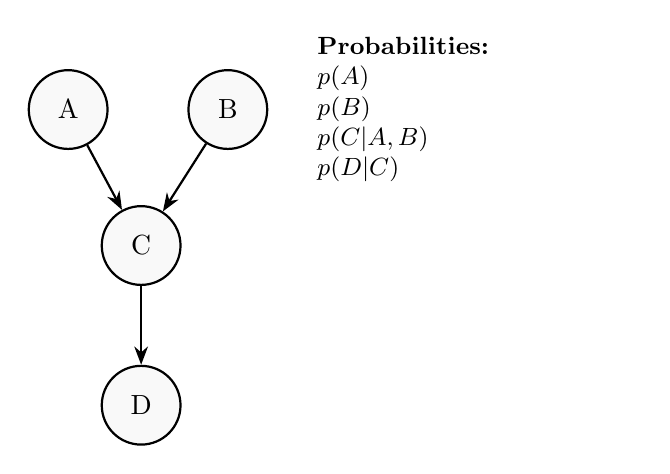
\begin{tikzpicture}[
                node distance=1cm,
                mynode/.style={draw, circle, minimum size=1cm, thick, fill=gray!5}
                ]

                % 노드 배치
                \node[mynode] (A) {A};
                \node[mynode] (B) [right=of A] {B};
                \node[mynode] (C) [below right=1cm and 0.2cm of A] {C};
                \node[mynode] (D) [below=of C] {D};

                % 에지 연결
                \draw[->, >=Stealth, thick] (A) -- (C);
                \draw[->, >=Stealth, thick] (B) -- (C);
                \draw[->, >=Stealth, thick] (C) -- (D);

                % 조건부 확률 표기 (노트)
                \node[right=0.5cm of B, text width=4cm, align=left, font=\small] {
                    \textbf{Probabilities:} \\
                    $p(A)$ \\
                    $p(B)$ \\
                    $p(C|A, B)$ \\
                    $p(D|C)$
                };
            \end{tikzpicture}
            \caption{Bayesian network}\label{fig:bayesianNet}
            \end{center}
        \end{figure}
        Figure \ref{fig:bayesianNet} represents the probability distribution $p(A, B, C, D) = p(D|C)p(C|A,B)p(B)p(A)$.
        We will discuss about graphical notations in next section.
    \subsection{Graphical Notations}
        TODO
    \subsection{Conditional Independences}
        \subsubsection{D-seperation}
            Before introducing the D-seperation method, which is useful for examing conditional independence properties of given
            bayesian network, we define some terminologies;
            \begin{itemize}
                \item head-to-head node with respect to path $a$: The node connects to the heads of the two arrows of the link in the path. 
                \item head-to-tail node with respect to path $a$: The node connects to the head and tail of two arrows of the link in the path.
                \item tail-to-tail node with respect to path $a$: The node connects to the tails of the two arrows of the link in the path.
                \item descendant of node \textbf{x}: There is a path to the node starting from \textbf{x}, considering the directions of the link.
            \end{itemize}

            \begin{thm}{D-seperation}{dSep}
                Consider a set of nodes $A$, $B$, and $C$, which does not intersect each other.
                Then, the path (ignoring the directions of links) from some element of $A$ to some element of $B$
                is \textbf{blocked} by $C$ if has node that satifies one of following two conditions:
                \begin{enumerate}
                    \item head-to-tail or tail-to-tail with respect to the path and belongs to $C$;
                    \item head-to-head with respect to the path or the descendant of such node and does not belong to $C$.  
                \end{enumerate}
                If every path is blocked, then the following conditional independence is satisfied:
                \[
                A \indep B\ | \ C
                \]
            \end{thm}

        \subsubsection{Markov Blanket}
            The \textbf{Markov blanket} is defined to be the nodes that make a given node to be conditionally
            independant to every other nodes when observed, i.e., the set of nodes $M_i$ that satisfy
            \[
            p(x_i, x_j|M_i)=p(x_i|M_i)p(x_j|M_i)
            \]
            for every $j$.
            In Bayesian network, the Markov blanket of node $x_i$ consists of:
            \begin{itemize}
                \item parents;
                \item children;
                \item and co-parent of children.
            \end{itemize} 
        
\section{Markov Random Field}
    \subsection{Definition}
        Before defining Markov random field, we define some concepts.
        \begin{defn}{Clique}{clique}
            \textbf{Clique} is a subset of nodes which have links connected to all the other nodes in the subset.
            \textbf{Maximal clique} is a clique which cannot add any more nodes without being clique anymore.
        \end{defn}

        Now we define Markov random field.
        \begin{defn}{Markov Random Field}{MRF}
            Let $G=(V,E)$ be an undirected graph. Then, the \textbf{Markov random field} with graph $G$ represents
            the following probability distribution:
            \[
            p(\textbf{x})=\frac{1}{Z}\prod_{C}\psi_C(\textbf{x}_C)
            \]
            where $C$ ranges over all maximal clique of $G$ and $\textbf{x}_C$ is all the node in $C$.
            \emph{partition function}, $Z$, is the constant that normalizes the equation so that it can represent
            a probability distribution.
            $\psi_C$ is called \emph{potential function}, and can be any function of $\textbf{x}_C$ with condition that
            it is positive or strictly positive.
        \end{defn}

    \subsection{Conditional Independence}
        \subsubsection{Conditional Independence in Markov Random Field}
            The conditional independence is easier to examine in Markov random field.
            \begin{thm}{Conditional Independence in Markov Random Field}{condIdepMRF}
                Let $A$, $B$, and $C$ be a set of nodes in Markov random field.
                Consider a path from $A$ to $B$. Then, the path is \textbf{blocked} by $C$
                if the path contains one or more nodes in $C$. If all path is blocked by, $C$,
                then $A \indep B\ | \ C$.
            \end{thm}
            Simple way is to think that $A \indep B\ | \ C$ when nodes in $A$ cannot reach any node in $B$
            if we delete all the nodes of $C$.
        \subsubsection{Markov Blanket}
            The Markov blanket of a given node in MRF is simply the adjacent nodes of a given node.

\section{$\mathcal I$-map, $\mathcal D$-map and $\mathcal P$-map}
    We now know how to represent probability distribution in terms of graphs, and we can do the opposite
    task, too. However, not all the probabilistic informations are preserved when converting from one to other.
    We propose a concept which describes this situation.
    \subsection{$\mathcal I$-map}
        \begin{defn}{$\mathcal I$-map}{iMap}
            Let $p(\mathbf{x})$ be a probability distribution. Then, the $\mathcal I$-map of the
            distribution is a graph whose conditional independencies are all satiesfied by the distribution.
        \end{defn}
        That is, \{probabilistic information of $\mathcal I$-map $\subset$ probabilistic information of $p(\mathbf{x})$\}.
    \subsection{$\mathcal D$-map}
        \begin{defn}{$\mathcal D$-map}{iMap}
            Let $p(\mathbf{x})$ be a probability distribution. Then, the $\mathcal D$-map of the
            distribution is a graph where all the conditional independencies in the distribution
            can be recognized from the graph itself.
        \end{defn}
        That is, \{probabilistic information of $p(\mathbf{x})$ $\subset$ probabilistic information of $\mathcal D$-map\}.
    \subsection{$\mathcal P$-map}
        \begin{defn}{$\mathcal P$-map}{iMap}
            Let $p(\mathbf{x})$ be a probability distribution. Then, the $\mathcal P$-map of the
            distribution is a graph which is simutaneously $\mathcal I$-map and $\mathcal D$-map
            of the distribution.
        \end{defn}
        That is, \{probabilistic information of $\mathcal P$-map = probabilistic information of $p(\mathbf{x})$\}.

\section{Inferences in Probabilistic Graphical Models}
    \href{run:../../inference/exact_inference/exact_inference.pdf}{See this document}.

\section{Application}
    \subsection{Linear-Gaussian Models}
        \begin{defn}{Linear-Gaussian Model}{LGModel}
            The \textbf{linear-Gaussian model} is a Bayesian network with following properties;
            \begin{itemize}
                \item Each node follows a Gaussian distribution.
                \item The mean of the Gaussian distribution is a linear combination of the parent nodes, i.e.,
                    $p(\mathbf{x}_i|pa_i)=\mathcal N \left(\textbf{x}_i \middle| \sum_{j \in pa_i}\mathbf{W}_{ij}\mathbf{x}_i + \mathbf{b}_i, \Sigma_i\right)$
            \end{itemize}
            Due to the properties of Normal distribution, the whole probability distribution $p(\textbf{x})$ is again a Normal distribution.
        \end{defn}
        The conjugate prior is a special case of the linear-Gaussian model.
    \subsection{Hidden Markov Model}
    \subsection{Linear Dynamic System} 
\end{document}